% INTRODUCCION

La parte superior de la atmósfera terrestre está siendo constantemente bombardeada con partículas provenientes del espacio, con energías de los $10^{10}\,$eV para arriba. Estas partículas son conocidas como rayos cósmicos (RC) y han sido medidas desde los años 60s \cite{linsley1961extremely}. Aunque el área lleva tiempo siendo estudiada, los mecanismos que producen los RCs y las zonas del espacio donde se originan los mismos siguen siendo investigadas por distintos experimentos. 


Por encima de una energía de $10^{14}\,$eV, los RCs que llegan a la atmósfera pueden interactuar con las moléculas de la misma,  y así producir cascadas de partículas secundarias. Dependiendo de la energía del primario, es decir el RC que generó la lluvia, estas partículas pueden ser medidas usando detectores sobre la superficie de la Tierra. Esta cascada es conocida como lluvia atmosférica extendida o \emph{EAS} y está compuesta por una componente electromagnética, que consiste en electrones, positrones y fotones, y una componente muónica. Las partículas secundarias cargadas también pueden excitar moléculas de nitrógeno en el aire que producen fotones de fluorescencia y pueden ser observados por telescopios durante noches claras.


El observatorio Pierre Auger está ubicado en la ciudad de Malargüe, provincia de Mendoza. El mismo fue construido para detectar las partículas secundarias de las EASs producidas por RCs, con energía por encima de $0.1\,$EeV. La adquisición de datos empezó en el año 2004. El observatorio posee un sistema híbrido de detección, ya que combina un arreglo de detectores de partículas sobre la superficie y un conjunto de telescopios que detectan los fotones de fluorescencia. Cuando el observatorio  registra una EAS que llega a la superficie y reconstruye la dirección de llegada del RC, se dice que se ha detectado un \textit{evento}.


Los análisis presentados en este trabajo fueron realizados con los eventos obtenidos por $\sim 1600$ detectores Cherenkov, dispuestos sobre de $\sim 3000\,\text{km}^2$ a  $1500\,$m entre sí. Un conjunto de 7 detectores adyacentes, es decir una en el medio y 6 en los lados, forman una celda hexagonal. Esta disposición de tanques se menciona como \textit{arreglo principal}.   Cada detector consiste en un tanque cilíndrico con 12 toneladas de agua ultra-pura de $1.2\,$m de alto. En la parte superior del tanque están instalados 3 foto-multiplicadores que monitorean la radiación Cherenkov en el agua. El conjunto del tanque y la electrónica de detección  se menciona durante este trabajo como \textit{Surface Detector} o \textit{SD}.  Cada detector está midiendo constantemente los fotones en el agua. Muchos de estos fotones son producidos por ruido y otros por partículas secundarias de una EAS. Los SDs cuentan con algoritmos o reglas para discernir ruido de un evento causado por un rayo cósmico, estos son los algoritmos de disparo.


\section{Acerca de todos los disparos del SD}

A medida que los tanques pasan más tiempo midiendo, también van perdiendo sensibilidad a los eventos de bajas energías. Esto es una desventaja del disparo estándar en los SDs en el rango $1\,$EeV - $2\,$EeV. En la Fig.\ref{fig:futuro}, para los datos presentados en el ICRC 2019, se observa como la energía media de los eventos para distintos rangos de tiempo va aumentando, además que la proporción de eventos por debajo de $3\,$ EeV disminuye. 

\begin{figure}[H]
	\centering
	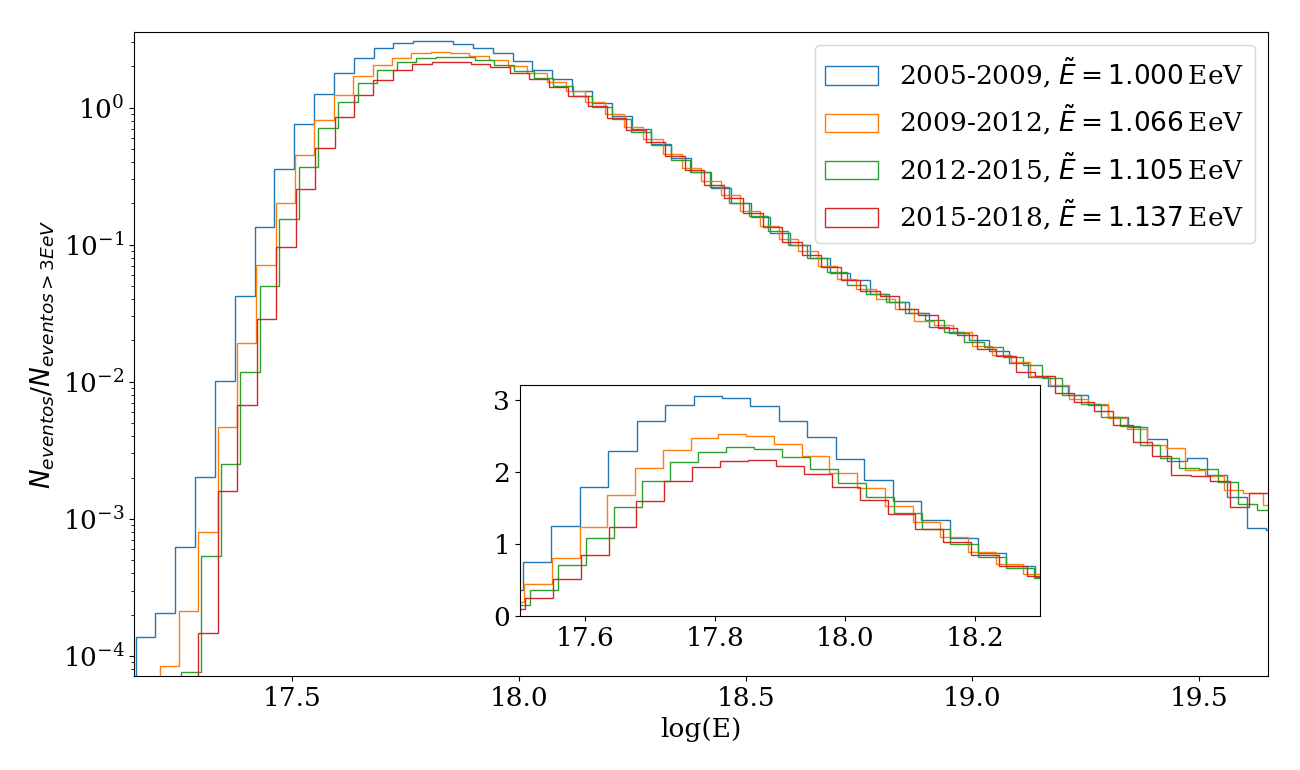
\includegraphics[width=0.8\textwidth]{histograma_evolucion_eventos.png}
	\caption{Histograma de eventos por rango de tiempo medido por el Observatorio Pierre Auger}
	\label{fig:futuro}
\end{figure}


El análisis del trabajo de licenciatura fue realizado sobre los eventos medidos utilizando el disparo estándar del arreglo principal, cuya eficiencia varía con la energía del CR. Para el disparo estándar, los eventos con energía mayor a $3\,$EeV y ángulo cenital $\theta_{max}<60^o$ o  por encima de $4\,$EeV y $\theta_{max}<80^o$, son detectados con una eficiencia del 100\%. Por lo tanto, el análisis en el rango de energía entre $1\,$EeV - $2\,$EeV requiere factores relacionados con la eficiencia del disparo en función de la energía. Estos factores son obtenidos de manera fenomenológica \cite{taborda}. 

Para superar esta dificultad y  poder recuperar la sensibilidad para bajas energías, a partir del año 2013  se implementó otros algoritmos de disparo en los SDs, llamados ToTd y MoPS \cite{pierre2013plans}. Estos algoritmos de disparo se mencionan en este trabajo como \textit{todos los disparos}. La implementación de los ToTd y MoPS fue llevada a cabo mediante una actualización de la electrónica de los SDs para bajar el umbral de disparo, en particular para las señales de la componente electromagnética de la EAS, mejorando así la reconstrucción de eventos mediante la separación fotón/hadrón para bajas energías  \cite{pierre2013plans}. Con esta mejora, la eficiencia completa se alcanza a partir de una energía mayor a $1\,$EeV. De tal manera que, al estudiar los eventos en el rango $1\,$EeV - $2\,$EeV,  no son necesarios los factores de eficiencia y sólo pueden afectar los cambios de la exposición direccional del observatorio.


Una desventaja de todos los disparos sobre el disparo estándar, es que el último tiene una mayor cantidad de años medidos en el rango $1\,$EeV - $2\,$EeV, ya que se adquieren datos  desde el año 2004 con este algoritmo. Esto es conveniente ya que mientras más años han sido medidos es más factible que los efectos espúreos se cancelen. En cambio, para todos los disparos, el análisis  es posible desde el año 2013. Entre inicios del 2004 y finales del 2019, el conjunto de eventos del disparo estándar tiene $6\,975\,194$ eventos sin clasificar. En cambio entre mediados del 2013 hasta fines del 2019, el archivo de eventos para todos los disparos tiene $13\,739\,351$ eventos sin clasificar, por lo que el menor tiempo de medición se compensa con la eficiencia del disparo.


\section{Acerca de los eventos} \label{filtro}

Se aplican cortes a los eventos para asegurar la eficiencia completa de los detectores. Estos cortes implican límites en ángulo cenital $\theta$ de los eventos, en la cantidad de vecinos al tanque de mayor señal, además de restringirse a eventos medidos en condiciones normales, es decir, cuando los sistemas de comunicación del Observatorio funcionan sin inconvenientes. De esta manera, podemos prescindir de otros factores de corrección.

A partir de los registros de eventos del arreglo principal con todos los disparos, se consideran solamente los eventos que cumplan las siguientes características:

    \begin{enumerate}
      \item La calidad de la reconstrucción depende de la energía y del ángulo cenital $\theta$ del evento.  Para eventos por debajo de los $4\,$EeV, se consideran los eventos con $\theta < 60^o$, en cambio para eventos por encima de esta energía se consideran hasta $\theta < 80^o$.
      \item Los datos del evento son recopilados sin inconvenientes. Este filtro se conoce como \emph{Bad period flag} o $ib$. Un valor de 1 indica un buen periodo. Con este filtro se descartan eventos debido a probables de alimentación o problemas de comunicación o adquisición que podrían inducir errores en el análisis.
      \item Buena reconstrucción de la lluvia atmosférica asociada al evento.
      \item El tanque de mayor señal está en el interior de un hexágono de tanques activos. Estos eventos se conocen como \textit{eventos 6T5}.
    \end{enumerate}


\subsection{Acerca del registro de hexágonos}\label{hexagonos_rate}

La cantidad de celdas  activas sobre el observatorio está relacionado con el filtro de eventos $6T5$, que garantiza la calidad de la reconstrucción del evento. El observatorio lleva un registro de la cantidad de hexágonos activos cada 5 min, además de registrar las condiciones atmosféricas en distintas estaciones de clima sobre la superficie del observatorio. 


\section{Acerca de la tesis de licenciatura}

Durante la tesis de licenciatura se analizaron los efectos de las condiciones atmosféricas durante el desarrollo de las EAS.  Se analizaron los datos adquiridos durante en el periodo 2005-2018 por el arreglo principal. De esta manera, se extendió los periodos estudiados anteriormente en los siguientes trabajos \cite{abraham2009atmospheric}, \cite{abreu2012description}   y \cite{aab2017impact}. 

Los efectos atmosféricos afectan principalmente a la atenuación de la componente electromagnética  de la EAS, en particular depende fuertemente de la temperatura y presión. Estos efectos  se caracterizan por parámetros dependientes del ángulo cenital del evento y por la presión, densidad y temperatura al momento de su detección. Los parámetros mencionados se utilizan para corregir las señales registradas por los SDs. Las correcciones del clima utilizadas por la colaboración Pierre Auger fueron implementadas a partir del trabajo \cite{aab2017impact} en el 2017. 

Durante el trabajo de la licenciatura se imitó el análisis de la modulación del clima sobre el periodo 2005-2015 del trabajo \cite{aab2017impact}, obteniéndose resultados compatibles. También se estudió la modulación del clima mediante el valor de la señal medida por los SDs, $S_{38}$, sin la corrección propuesta por \cite{aab2017impact}, además de extender el rango de tiempo analizado hasta el 2018. Se observó que los parámetros del clima obtenidos en este análisis sobre  $S_{38}$  son compatibles con los utilizados en la reconstrucción oficial. 